\documentclass{article}
\usepackage{tikz}
\usepackage[utf8]{inputenc}
\usepackage{amsfonts}
\usetikzlibrary{automata,positioning}

\title{Autómatas y lenguajes formales. Tarea 1}
\author{Fabián Romero Jiménez}
\begin{document}
\maketitle
\begin{enumerate}
\item Las listas de números naturales $L( \mathbb{N} )$ se pueden definir a partir de un elemento básico, la lista vacía
$$ [ ] $$
y la función ::, que toma números naturales y listas y da por resultado nuevas listas. Por ejemplo, si $ n \in \mathbb{N}$ y $[n_{1} . . . n_{m}] \in L(\mathbb{N}) $, entonces $$ n :: [n_{1} . . . n_{m}] = [n n_{1} . . . n_{m}] $$
Considera ahora las funciones $ Sum : L(\mathbb{N}) \rightarrow \mathbb{N} $ y $ doble : L(\mathbb{N}) \rightarrow L(\mathbb{N}) $
$$ Sum([ ]) = 0     $$
$$ Sum(n :: l) = n + Sum(l)   $$
$$ doble([ ]) = [ ] $$
$$ doble(n :: l) = (2  n) :: (doble(l)) $$
Demuestra por inducción que $ 2 \times Sum(l) = Sum(doble(l))$ para toda lista finita l.

\textbf{Demostración:}\\
Para el caso de $n = 0$ tenemos que demostrar:
$$  2 \times Sum([]) = Sum(doble([]))  $$
dado que $ Sum([ ]) = 0  $
$$  2 \times 0 = Sum(doble([]))  $$
y usando que $ doble([ ]) = [ ] $ y tambien que $ Sum([ ]) = 0  $
$$  2 \times 0 = Sum([])= 0 $$

Con lo que queda concluido el caso base.
Luego, asumamos que es cierto para  $k$
i.e
$$  2 \times Sum(l) = Sum(doble(l)) $$ para toda lista l de longitud $k$
Entonces, sea $l_{k+1}$ una lista cualquiera de longitud $k+1$, por lo que podemos entenderla como $n::l$, donde $n$ el el primer elemento de la lista y l una lista de longitud k, por lo que por hipotesis de inducción tenenos:
$$  2 \times Sum(l) = Sum(doble(l))  $$
y tambien sabemos que $ Sum(n::l)=n + Sum(l) $ de lo que se desprende que 
$$ Sum(l_{k+1}) = Sum(n::l)=n + Sum(l) =  $$ 
sabemos que $Sum(n::l) =$

\end{enumerate}
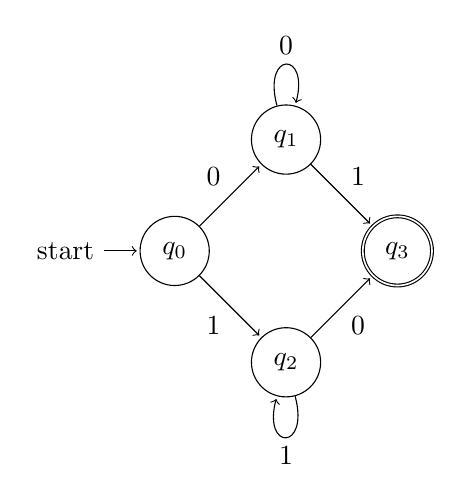
\begin{tikzpicture}[shorten >=1pt,node distance=2cm,on grid,auto] 
   \node[state,initial] (q_0)   {$q_0$}; 
   \node[state] (q_1) [above right=of q_0] {$q_1$}; 
   \node[state] (q_2) [below right=of q_0] {$q_2$}; 
   \node[state,accepting](q_3) [below right=of q_1] {$q_3$};
    \path[->] 
    (q_0) edge  node {0} (q_1)
          edge  node [swap] {1} (q_2)
    (q_1) edge  node  {1} (q_3)
          edge [loop above] node {0} ()
    (q_2) edge  node [swap] {0} (q_3) 
          edge [loop below] node {1} ();
\end{tikzpicture}
\end{document}  

%como un truco sencillo para beneficiarse de la ignorancia y credibilidad de algunos ingenuos?
%Demostremos por inducción sobre la longitud de la lista.
%
%Caso base, lista vacia L=[]:
%Por definición
%Sum([])=0, double([])=[]
%asi que:
%2 x Sum([]) = 2 x 0 = 0
%Sum(double(L))=Sum([])=0
%
%Supongamos que 2 x Sum(l) = Sum(doble(l)) se cumple para todas las listas de longitud hasta n-1.
%
%sea l una lista de longitud n que es el elemento k seguido de la lista de longitud n-1 l1
%2 x Sum(L)=2 x Sum(k::l1)= 2 x (k + Sum(l1)) =2 X k + 2 x Sum(l1) = Sum(double(n::l1)) QED
